\chapter[Limits of Convolutional Neural Networks on FLS Images]{Limits of Convolutional \newline Neural Networks on FLS Images}
\label{chapter:limits}

This chapter deals with a less applied problem than the rest of this thesis. While the use of Deep Neural Networks for different tasks has exploded during the last 5 years, many questions of practical importance remain unanswered \cite{zhang2016understanding}.

A general rule of thumb in machine learning is that more data always improves the generalization ability of a classifier or regressor. For Deep Learning it has been largely assumed that a large dataset is required. But experiments done in this thesis, specially in the previous chapter, show that CNNs can be trained with smaller datasets.

A big problem is then defining what is a "large" or a "small" dataset. In the computer vision community, a large dataset might be ImageNet \cite{russakovsky2015imagenet} with 1.2 million images and 1000 labeled classes, while for the marine robotics community 2000 images might be large, and 200 images with 2-4 classes might be small.

A very common requirement by practitioners is an estimate of how many data points are required to solve a given learning task. Typically as data needs to be gathered, an estimate of how much data is needed would be quite useful. Other effects are also of interest, such as what is the optimal object size for recognition, and what are the best ways to perform transfer learning, and how does that affect the training set size that is required for a given performance target.

In this chapter we would like to explore the following research questions:

\begin{itemize}
	\item How does object size affect classification performance? Can small objects be recognized similarly to bigger ones?
	\item How much data is required for FLS classification?
	\item How can networks be made to require less training data given a classification performance target.
	\item How effective is transfer learning in features learned from sonar images?
\end{itemize}

We try to answer these questions from an experimental point of view, by performing different synthetic experiments on our dataset of marine debris objects.

\section{Related Work}

Surprisingly, there is little literature about these research questions, even as they are quite important for practitioners.

Sharif et al. \cite[-3em]{sharif2014cnn} was one of the first to evaluate features learned by a CNN. They used a pre-trained OverFeat \cite[1em]{sermanet2013overfeat} as a feature extractor network, and computed features from the fc1 \footnote[][1em]{First fully connected layer} layer, which corresponds to a $4096$ long vector. This vector is then normalized with the L2 norm and used to train a multi-class SVM. An additional combination using data augmentation is also explored by the authors.

On the PASCAL VOC 2007 dataset, this method obtains better accuracy for 14 out of 21 classes, with a slightly worse accuracy on 7 classes. Note that the state of the art compared in this work is mostly composed of engineered features, like bag of visual words, clustering, and dictionary learning from HoG, SIFT and LBP features. Even as OverFeat is not trained on the same dataset, its features generalize outside of this set quite well.

On the MIT 67 indoor scenes dataset, the authors obtain $69.0$ \% mean accuracy with data augmentation, which is $5$ \% better than the state of the art. This dataset is considerably different from the ImageNet dataset used to train OverFeat.

In order to evaluate a more complex task, the authors used the Caltech-UCSD Birds dataset, where the task is to classify images of 200 different species of birds, where many birds "look alike" and are hard to recognize. Again this simple method outperforms the state of the art by $6$ \%, producing $61.8$ accuracy. This result shows how CNN features outperform engineered ones, even when the task is considerably different from the training set.
This work also shows the importance of data augmentation for computer vision tasks.

Pailhas, Petillot and Capus \cite[-3em]{pailhas2010high} have explored the relationship between sonar resolution and target recognition accuracy. While this is not the same question as we are exploring, it is similar enough to warrant inclusion in this state of the art. This work concentrates on the sonar resolution as a physical property of the device itself, while we want to explore this relation from the image processing point of view.

The authors use a sidescan sonar simulator that produces synthetic sonar images. The background that were considered are a flat seabed, sand ripples, a rocky seabed, and a cluttered environment (rocks). The target are mine-like objects, including six classes (manta, rockan, cuboid, hemisphere, a lying cylinder on the side and a standing one).

The classifier used in this work is based on a Principal Component Analysis representation, that is matched with templates in a training set by means of minimizing a distance in feature space. The authors analyse the use of shadow or highlight features.

For classification using highlight, $95$ \% accuracy is obtained with 5 cm pixel resolution, which is considerably fine grained for a sidescan sonar. In contrast, classification using shadow requires less than 20 cm pixel resolution to obtain close to $100$ \% accuracy, but highlight classification at 20 cm pixel resolution is close to $50$ \%.
This work shows that using the shadow of an object is fundamental for good classification performance, but we believe these results are skewed due to the use of a PCA-based classifier. Other classifiers might perform differently. There is also the issue of the objects used in this work, as marine debris is considerably different in shape variation and lack of shadow information.

Mishkin et al. \cite{mishkin2016systematic} do a systematic evaluation of many network parameters for the ImageNet dataset in the context of image classification. This work consists of a large number of ablation studies, varying activation functions, different kinds of pooling, learning rate policies, pre-processing and normalization, batch size, etc.

Two results from these work are of interest for this chapter. The authors evaluated the effect of varying the input image size, which shows that decreasing the input image has the effect of reducing accuracy from $50$ \% at $224 \times 224$ input size to $30$ \% at $66 \times 66$ pixels. The relationship between input image size and accuracy is almost linear.
One way to offset this loss is to vary the network architecture as a function of the input size, as the authors tried to vary the strides and filter sizes to produce a constant size pooling output, reducing the effect of image size as accuracy only varies from $40$ \% to $45$ \%.

The second result is the variation of the training set size. The authors down-sample the ImageNet dataset to $0.2$ M, $0.4$ M, $0.6$ M, $0.8$ M and 1.2 million images (the original size). Accuracy decreases from $45$ \% at $1.2$ M to $30$ \% at $0.2$ M. The relationship between training set size and accuracy is quite close to linear, as it slowly decreases linearly from $1.2$ M to $0.4$ M, but then decreases more sharply.
While both results are quite interesting, these authors have not controlled for the random weight initialization, and variations of accuracy should be computed. Due to the large size of the ImageNet dataset, it can expected that these kind of evaluation protocol is not available due to the large computational resources required.

\section{Transfer Learning}
\label{lim:secTransferLearning}

In this experiment we evaluate the transfer learning capabilities of three networks we designed: ClassicNet, TinyNet and FireNet.

Our general procedure to evaluate transfer learning in a network is to first define a set of layers $L$ that we wish to evaluate. The features produced as output from these layers are then used to train a multi-class SVM \cite{sharif2014cnn}. In order to produce a fair evaluation of the features, we decided to split the training and testing sets according to the classes they contain, in order to learn features on one set of objects and test them in a different set of objects.
This should aid to verify the generalization capabilities of the network architecture.

We first split the dataset $D$ into datasets $F$ and $T$ by selecting a random subset of $\lfloor \frac{C}{2} \rfloor$ classes and assigning all samples from those classes to $F$, while the remaining classes and their samples are assigned to $T$. As our Marine Debris dataset contains 11 samples, 6 classes are assigned to $F$ and 5 are assigned to $T$. We split both the training and testing splits of our dataset separately, producing $F_{tr}$, $F_{ts}$ and $T_{tr}$, $T_{ts}$.

Dataset $F$ is to learn features by training a network model for classification, while $T$ is used to evaluate features. A given network model is trained on $F_{tr}$ and then for each layer in $L$, features are extracted at that layer from the network model by passing each sample in $T_{tr}$. Then a multi-class linear SVM with regularization coefficient $C = 1$  and decision surface "one-versus-one" is trained on those features \footnote{$C$ was obtained by cross-validation on a small part of the dataset}. Using the same network, features are again extracted using $T_{ts}$ and the SVM is tested on this dataset, producing an accuracy score. We repeat this process $N = 20$ times to account for random initialization of the feature extraction network and compute mean and standard deviation of test accuracy. Note that $F_{ts}$ is not used by this procedure, but it could be used to evaluate test accuracy of the feature extractor.

ClassicNet with 5 modules was tested with four different configurations: 8 or 32 filters, and Batch Normalization or Dropout as regularization. Features are extracted from the batch normalized outputs in each module (layers bn1-5), or from the Max-Pooling outputs in the case of the Dropout configurations (layers mp1-5), and we also include the output from the first fully connected layer (fc1). We used TinyNet with 5 modules and 8 filters per module, and FireNet with 3 modules and 4 filters. For TinyNet, features are extracted at the output of each of the five modules, while for FireNet features are the outputs of each module (three in total) and we also consider the output of the initial convolution (called convS in the figures). Each feature extraction network is trained for 15 epochs with a batch size $B = 64$ using the ADAM optimizer \cite{kingma2014adam} with a learning rate $\alpha = 0.01$. The data is randomly shuffled after each epoch in order to prevent spurious patterns in the data ordering to influence the network.

Our results are shown in Figure \ref{lim:transferLearningNetworks}. A general pattern that appears in all three experimental plots is that testing accuracy decreases with deeper layers/modules in the network. For example, in ClassicNet, features in the fc1 layer have lower accuracy than bn1 and bn2. The same effect can be seen in TinyNet and FireNet, specially as the last module/layer has the lowest testing accuracy. It is also notable that the features in the first layers have $100$ \% accuracy, with zero variation. This can be explained that as shallow features are typically very high dimensional, a linear SVM has a high chance of finding a separating hyperplane and perfectly classifying test data.

ClassicNet feature results are shown in Figure \ref{lim:transferLearningNetworks}\subref*{lim:transferLearningNetworks:classic}. Generalization varies considerably with different layers. 8 filters with Batch Normalization produces quite good generalization, but 32 filters with Dropout has almost the same accuracy, with it being superior for bn5 and fc1. Dropout with 8 filters has a considerable drop in accuracy compared with the other configurations. 32 filters with Dropout seems to be the best option for good generalization, which is consistent with the use of Dropout to both de-correlate neurons and increase their generalization power \cite{srivastava2014dropout}.

\begin{figure*}
	\subfloat[ClassicNet]{
		\label{lim:transferLearningNetworks:classic}
		\begin{tikzpicture}
		\begin{axis}[ybar,
		xlabel={Layers},
		ylabel={Test Accuracy (\%)},        
		symbolic x coords={bn1, bn2, bn3, bn4, bn5, fc1},
		xtick=data,
		legend style={at={(0.5,1.15)},anchor=north,legend columns=-1},
		ymajorgrids=true,
		grid style=dashed,
		height = 0.3\textheight,
		width = 0.9\textwidth]
				
		\addplot+[error bars/.cd, y dir=both,y explicit] table[x = layerIdx, y = meanTransferAcc, y error = stdTransferAcc, col sep = space] {chapters/data/limits/transferLearning-disjoint-ClassicNet-BN-5modules-8filters.csv};
		\addplot+[error bars/.cd, y dir=both,y explicit] table[x = layerIdx, y = meanTransferAcc, y error = stdTransferAcc, col sep = space] {chapters/data/limits/transferLearning-disjoint-ClassicNet-BN-5modules-32filters.csv};
		
		\addplot+[error bars/.cd, y dir=both,y explicit] table[x = layerIdx, y = meanTransferAcc, y error = stdTransferAcc, col sep = space] {chapters/data/limits/transferLearning-disjoint-ClassicNet-DO-5modules-8filters.csv};
		\addplot+[error bars/.cd, y dir=both,y explicit] table[x = layerIdx, y = meanTransferAcc, y error = stdTransferAcc, col sep = space] {chapters/data/limits/transferLearning-disjoint-ClassicNet-DO-5modules-32filters.csv};
		
		\legend{8 filters with BN, 32 filters with BN, 8 filters with Dropout, 32 filters with Dropout}
		
		\end{axis}
		\end{tikzpicture}		
	}
	
	\subfloat[TinyNet]{
		\label{lim:transferLearningNetworks:tiny}
		\begin{tikzpicture}
		\begin{axis}[ybar,
		xlabel={Modules},
		ylabel={Test Accuracy (\%)},        
		xtick=data,
		legend style={at={(0.5,1.15)},anchor=north,legend columns=-1},
		ymajorgrids=true,
		grid style=dashed,
		height = 0.3\textheight,
		width = 0.45\textwidth]
		
		\addplot+[error bars/.cd, y dir=both,y explicit] table[x = layerIdx, y = meanTransferAcc, y error = stdTransferAcc, col sep = space] {chapters/data/limits/transferLearning-disjoint-tinyNet5-8.csv};
		
		\end{axis}
		\end{tikzpicture}
	}
	\subfloat[FireNet]{
		\label{lim:transferLearningNetworks:fire}
		\begin{tikzpicture}
		\begin{axis}[ybar,
		xlabel={Layers},
		ylabel={Test Accuracy (\%)},        
		symbolic x coords={convS, mod1, mod2, mod3},
		xtick=data,
		legend style={at={(0.5,1.15)},anchor=north,legend columns=-1},
		ymajorgrids=true,
		grid style=dashed,
		height = 0.3\textheight,
		width = 0.45\textwidth]
		
		\addplot+[error bars/.cd, y dir=both,y explicit] table[x = layerIdx, y = meanTransferAcc, y error = stdTransferAcc, col sep = space] {chapters/data/limits/transferLearning-disjoint-fireNet3.csv};
		
		\end{axis}
		\end{tikzpicture}
	}
	
	\vspace*{0.5cm}
	\caption[Transfer Learning on Sonar Images]{Transfer Learning on Sonar Images. Mean test accuracy produced by an SVM trained on features output by different layers. Three networks are shown.}
	\label{lim:transferLearningNetworks}
\end{figure*}

Results for TinyNet are shown in Figure \ref{lim:transferLearningNetworks}\subref*{lim:transferLearningNetworks:tiny}, and for FireNet in Figure  \ref{lim:transferLearningNetworks}\subref*{lim:transferLearningNetworks:fire}. The shape of both plots is quite similar, with a decrease from the first to the second module, and then a increase, followed by another decrease. Seems using the layer before the last might have the best generalization performance, but using the first layer has by far the best accuracy.

It should be noted that for both TinyNet and FireNet, their generalization capability is very good, with the minimum accuracy being greater than $96$ \%. Our results also seem to indicate that choosing features from the last layer might not always be the best option, as it has consistently been done by many researchers. This could be a peculiarity of sonar images, and we do not believe it applies for larger datasets.

As summary, we expected that transfer learning using CNN features will perform adequately and it did, but it was unexpected that we found negative correlation between layer depth and test accuracy, For this kind of data and architecture, the best choice is to extract a high dimensional feature vector from a layer close to the input.

\begin{marginfigure}
	\centering
	\stackunder[5pt] {
		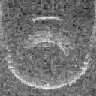
\includegraphics[width = 3cm]{tire-96x96.jpg}
	}{$96 \times 96$}

	\vspace{5pt}
	
	\stackunder[5pt] {
		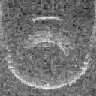
\includegraphics[width = 2.5cm]{tire-96x96.jpg}
	}{$80 \times 80$}
	
	\vspace{5pt}
	
	\stackunder[5pt] {
		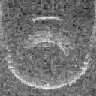
\includegraphics[width = 2.0cm]{tire-96x96.jpg}
	}{$64 \times 64$}
	
	\vspace{5pt}
	
	\stackunder[5pt] {
		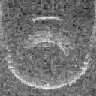
\includegraphics[width = 1.5cm]{tire-96x96.jpg}
	}{$48 \times 48$}
	
	\vspace{5pt}
	
	\stackunder[5pt] {
		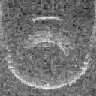
\includegraphics[width = 1.0cm]{tire-96x96.jpg}
	}{$32 \times 32$}
	
	\vspace{5pt}
	
	\stackunder[5pt] {
		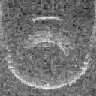
\includegraphics[width = 0.5cm]{tire-96x96.jpg}
	}{$16 \times 16$}
	
	\caption[Example of object scales used for our experiment]{Example of object scales used for our experiment. These images correspond to a Tire.}
\end{marginfigure}

\FloatBarrier
\section{Effect of Object Size}

In this section we experiment with object size, as we would like to investigate how the object size/scale affects classification accuracy.

For this purpose we take the initial $96 \times 96$ image crops and downscale them using bilinear filtering to a predefined size. We use square pixel sizes $s \times s$ with $s \in [16, 32, 48, 64, 80, 96]$. To obtain the size parameters, we started from the natural size of the bounding boxes in our dataset ($96 \times 96$ pixels) and downscaled them in 16 pixel steps, until we reached the smallest size that can be classified by a 2-module ClassicNet, which is 16 pixels (due to downsampling by the use of Max-Pooling). Both the training and testing sets are resized. We evaluate accuracy on the test set. In order to account for the effect of random initialization, we train $N = 20$ networks and compute the mean and standard deviation of accuracy.

We found experimentally \cite{valdenegro2017limits} that the kind of regularization and optimizer that are used greatly affect the results. We evaluate four combinations, using Batch Normalization or Dropout for regularization, and ADAM or SGD for optimizer. All networks for every configuration are trained for $30$ epochs, using a learning rate $\alpha = 0.01$ with a batch size $B = 128$ samples.

We selected three networks to be evaluated: ClassicNet with 2 modules and 32 filters, TinyNet with 5 modules and 8 filters, and FireNet with 3 modules and 4 filters. We only evaluate ClassicNet with both Batch Normalization and Dropout, as it is not appropriate to use Dropout with a fully convolutional network such as TinyNet and FireNet. In these two networks we only use Batch Normalization as regularizer.  

We present our results as a plot in Figure \ref{lim:graphicalObjectSize} and as numerical values in Table \ref{lim:numericalObjectSize}. For ClassicNet, we can see that a high accuracy classifier is produced by using both ADAM and Batch Normalization. ADAM with Dropout also produces quite high accuracy but lower than using Batch Normalization. Using SGD produces considerably lower accuracy classifiers, specially when combined with Dropout.

One of the results we expected is that accuracy should decrease with smaller object size, as less information is available for the classifier and its typical that smaller objects are harder to classify. Our results show that this happens when using SGD on ClassicNet, as accuracy monotonically increases as object size also increases. This is more noticeable with the SGD-Dropout configuration.

But unexpectedly, the ADAM combinations produce high accuracy that seems to be invariant to object size. The ADAM with Batch Normalization combination consistently produces results that are very accurate (only $1.5$ \% from perfect classification) with little variation.

\begin{table*}[!ht]
    \centering
	\forceversofloat
	\begin{tabular}{llll}
		\hline 
		Model / Pixel Size 			& 16 				   & 32 				    & 48\\ 
		\hline
		ClassicNet-ADAM-BN  & $98.5 \pm 0.5$ \%    & $98.6 \pm 0.3$ \%  & $98.5 \pm 0.3$ \%\\
		ClassicNet-SGD-BN 	& $85.7 \pm 2.6$ \%    & $85.6 \pm 2.7$ \%  & $89.9 \pm 4.7$ \%\\
		ClassicNet-ADAM-DO  & $91.5 \pm 1.5$ \%    & $96.6 \pm 0.9$ \%  & $97.2 \pm 0.6$ \%\\
		ClassicNet-SGD-DO 	& $13.9 \pm 2.6$ \%    & $18.2 \pm 5.5$ \%  & $22.3 \pm 5.8$ \%\\
		\hline
		TinyNet-ADAM-BN 	& $95.8 \pm 1.1$ \%    & $95.2 \pm 1.6$ \%  & $93.7 \pm 1.6$ \%\\
		TinyNet-SGD-BN 	    & $70.2 \pm 9.7$ \%    & $54.2 \pm 10.0$ \% & $39.7 \pm 10.0$ \%\\
		\hline
		FireNet-ADAM-BN  	& $93.7 \pm 2.9$ \%    & $96.7 \pm 0.7$ \%  & $96.1 \pm 1.0$ \%\\
		FireNet-SGD-BN 		& $76.9 \pm 7.5$ \%    & $62.6 \pm 9.5$ \%  & $56.0 \pm 11.1$ \%\\
		\hline 
	\end{tabular}
    \begin{tabular}{llll}
        \hline 
        Model / Pixel Size 			& 64 				  & 80 				& 96\\ 
        \hline
        ClassicNet-ADAM-BN  & $98.1 \pm 0.3$ \% & $98.2 \pm 0.5$ \% & $98.1 \pm 0.5$ \%\\
        ClassicNet-SGD-BN 	& $90.1 \pm 1.5$ \% & $93.6 \pm 1.0$ \% & $95.1 \pm 1.0$ \%\\
        ClassicNet-ADAM-DO  & $96.5 \pm 0.7$ \% & $97.1 \pm 0.6$ \% & $97.5 \pm 0.5$ \%\\
        ClassicNet-SGD-DO 	& $26.1 \pm 7.2$ \% & $39.1 \pm 10.0$ \% & $47.3 \pm 9.5$ \%\\
        \hline
        TinyNet-ADAM-BN 	& $89.3 \pm 5.2$ \% & $88.7 \pm 6.0$ \% & $85.0 \pm 9.1$ \%\\
        TinyNet-SGD-BN 	    & $36.9 \pm 6.9$ \% & $31.2 \pm 9.0$ \% & $33.0 \pm 5.7$ \%\\
        \hline
        FireNet-ADAM-BN  	& $92.1 \pm 2.2$ \% & $90.0 \pm 2.5$ \% & $91.1 \pm 2.6$ \%\\
        FireNet-SGD-BN 		& $46.8 \pm 7.3$ \% & $45.4 \pm 6.4$ \% & $45.6 \pm 7.5$ \%\\
        \hline 
    \end{tabular}
    \vspace*{0.5cm}
	\caption{Numerical summary of the effect of object size/scale for different CNN models.}
	\label{lim:numericalObjectSize}
\end{table*}

TinyNet and FireNet results are not as good as ClassicNet. Both networks seem to have a negative correlation with object size, starting from high accuracy for small objects, and decreasing the precision of their predictions as objects gets bigger. This was quite unexpected. We believe this result can be explained by the fact that as these networks have a considerably lower number of parameters, the number of "acceptable" or "right" values for the weights is smaller, and thus these networks require more data in order to generalize properly.
Comparing these results with Chapter \ref{chapter:sonar-classification}, where we used data augmentation, we can see that not using data augmentation as we do here considerably reduces classifier generalization.
Using ADAM produces acceptable accuracy, but it still decreases slightly with bigger objects. These results also show that FireNet can be considerably more accurate than TinyNet, probably owning to the larger number of parameters.

Our combined results show that the combination of both ADAM and Batch Normalization produce a very good classifier that seems to be invariant to object size. This can be explained as both ADAM and Batch Normalization are adaptive algorithms. ADAM adapts the learning rate with the exponentially running mean of the gradients, so when the optimization process is close to a high-accuracy minima, it can adapt the learning rate in order to consistently reach that minima. SGD alone cannot do this, even if fixed learning rate schedules are used. Gradient information as part of learning rate calculation is a key for this process to succeed.

As a general summary of these results, it is possible to say that a convolutional neural network can be designed and trained in a way that it is approximately invariant to object size. This requires the use of an adaptive learning rate (ADAM) and an appropriate regularization and control of the co-variate shift throught the use of Batch Normalization. Dropout combined with ADAM also produces a size invariant classifier but it is less accurate than other configurations.

\begin{figure*}
	\subfloat[ClassicNet]{
		\begin{tikzpicture}
		\begin{axis}[
		xlabel={Image size (Pixels)},
		ylabel={Test Accuracy (\%)},        
		ymin=10, ymax=100,
		xtick={16, 32, 48, 64, 80, 96},
		ytick={20,30,40,50,60,70,80,90,100},
		legend style={at={(0.5, 1.05)},anchor=south},
		ymajorgrids=true,
		grid style=dashed,
		height = 0.3\textheight,
		width = 0.45\textwidth]
		
		\errorband{chapters/data/limits/classicCNN-BN-ADAM-AccuracyVsImageSize.csv}{pixelImageSize}{meanAcc}{stdAcc}{blue}{0.4}
		\errorband{chapters/data/limits/classicCNN-BN-SGD-AccuracyVsImageSize.csv}{pixelImageSize}{meanAcc}{stdAcc}{red}{0.4}
		
		\errorband{chapters/data/limits/classicCNN-Dropout-ADAM-AccuracyVsImageSize.csv}{pixelImageSize}{meanAcc}{stdAcc}{green}{0.4}
		\errorband{chapters/data/limits/classicCNN-Dropout-SGD-AccuracyVsImageSize.csv}{pixelImageSize}{meanAcc}{stdAcc}{magenta}{0.4}
		
		\legend{ADAM-BN, SGD-BN, ADAM-Dropout, SGD-Dropout}
		
		\end{axis}
		\end{tikzpicture}
	}
	\subfloat[TinyNet and FireNet]{
		\begin{tikzpicture}
		\begin{axis}[
		xlabel={Image size (Pixels)},
		ylabel={Test Accuracy (\%)},        
		ymin=10, ymax=100,
		xtick={16, 32, 48, 64, 80, 96},
		ytick={20,30,40,50,60,70,80,90,100},
		%ytick={0,20,40,60,80,100,120},
        legend style={at={(0.5, 1.05)},anchor=south},
		ymajorgrids=true,
		grid style=dashed,
		height = 0.3\textheight,
		width = 0.45\textwidth]
		
		\errorband{chapters/data/limits/tinyNetCNN-BN-AccuracyVsImageSize.csv}{pixelImageSize}{meanAcc}{stdAcc}{blue}{0.4}
		\errorband{chapters/data/limits/tinyNetCNN-BN-SGD-AccuracyVsImageSize.csv}{pixelImageSize}{meanAcc}{stdAcc}{red}{0.4}
		
		\errorband{chapters/data/limits/smallFireNetCNN-BN-AccuracyVsImageSize.csv}{pixelImageSize}{meanAcc}{stdAcc}{green}{0.4}
		\errorband{chapters/data/limits/smallFireNetCNN-BN-SGD-AccuracyVsImageSize.csv}{pixelImageSize}{meanAcc}{stdAcc}{magenta}{0.4}
		
		\legend{TinyNet-ADAM-BN, TinyNet-SGD-BN, FireNet-ADAM-BN, FireNet-SGD-BN}
		
		\end{axis}
		\end{tikzpicture}
	}
	
	\vspace*{0.5cm}
    \forceversofloat
	\caption[Graphical summary of the effect of object size/scale for different CNN models]{Graphical summary of the effect of object size/scale for different CNN models. The shaded areas represent one $\sigma$ error bars.}
	\label{lim:graphicalObjectSize}
\end{figure*}

\FloatBarrier
\section{Effect of Number of Training Samples}
\label{lim:secNumTrainingSamples}

In this section we investigate how many training samples are required for a given generalization target. We do this by a simple but powerful experiment.

The basic idea of this experiment is to take a given training set $T$ and produce sub-sampled version of that dataset. As we are approaching a classification problem, we decided to normalize the number of image samples in each class (abbreviated SPC). We decide a set of SPC values and produce several sub-sampled versions of $T$, where for $T_{i}$ the number of samples per class in that dataset is $i$. This allows comparisons using different SPC values. The testing set is not sub-sampled in anyway in order to enable comparisons. Note that as our dataset is not balanced, and using this procedure will produce a balanced training set, so it is expected that the results will not match the ones from Chapter \ref{chapter:sonar-classification}, but as we are using the same testing set, results are comparable.

As it has been previously done, in order to consider the effect of random initialization, we train $N = 10$ instances of the same network model on each dataset $T_{i}$, but also we must consider the variations in the sub-sampled training set, as sampling is performed randomly. Then we also generate $M = 10$ different training sets with the same value of SPC, and train $N$ networks on each of these sets. After both variations are taken into account, we will train $N \times M = 100$ networks for each value of SPC.

We selected $\text{SPC} \in \{ [1, 2, 3, ..., 20] \cup [25, 30, 35, ..., 50] \cup [60, 70, 80, \newline ..., 150] \}$. The first range is designed to show the differences in generalization with small samples of data, while the other ranges show behaviour with large samples. As our dataset is unbalanced, we only evaluate up to 150 samples per class, which is only two times the number of samples of the class with the least samples.

We evaluate three networks, as it has previously been done: ClassicNet with 2 modules and 32 filters, combined and Batch Normalization and Dropout as regularizers. TinyNet with 5 modules and 8 filters, and FireNet with 3 modules and 4 filters. We have also included a linear SVM with $C = 10$ as a comparison baseline.

\begin{figure*}[t]
	\forcerectofloat
	\centering
	\begin{tikzpicture}
	\begin{customlegend}[legend columns = 4,legend style = {column sep=1ex}, legend cell align = left,
	legend entries={2 Modules-BN, 2 Modules-Dropout, SVM}]
	\addlegendimage{mark=none,blue}
	\addlegendimage{mark=none,red}
	
	\addlegendimage{mark=none,green}
	\end{customlegend}
	\end{tikzpicture}
	
	\subfloat[Full Plot]{
		\begin{tikzpicture}
		\begin{axis}[
		xlabel={Samples per Class},
		ylabel={Test Accuracy (\%)},        
		xmax = 150,
		ymin=35, ymax=100,
		xtick={1,10,20,30,40,50,60,70,80,90,100,110,120,130,140,150},
		ytick={30,40,50,60,70,80,90,95,100},
		x tick label style={font=\tiny, rotate=90},
		legend pos=south east,
		ymajorgrids=true,
		grid style=dashed,
		height = 0.25\textheight,
		width = 0.45\textwidth]
		
		\errorband{chapters/data/limits/classicCNN2L-BN-AccuracyVsTrainSetSize.csv}{samplesPerClass}{meanAcc}{stdAcc}{blue}{0.4}
		\errorband{chapters/data/limits/classicCNN2L-Dropout-AccuracyVsTrainSetSize.csv}{samplesPerClass}{meanAcc}{stdAcc}{red}{0.4}
		
		\errorband{chapters/data/SVM-C10-AccuracyVsTrainSetSize.csv}{samplesPerClass}{meanAcc}{stdAcc}{green}{0.4}
		
		\end{axis}
		\end{tikzpicture}
	}
	\subfloat[Zoom into region SPC $1-30$]{
		\begin{tikzpicture}
		\begin{axis}[
		xlabel={Samples per Class},
		ylabel={Test Accuracy (\%)},        
		xmin=1, xmax=30,
		ymin=35, ymax=100,
		xtick={1,2,3,4,5,6,7,8,9,10,11,12,13,14,15,16,17,18,19,20,25,30},
		ytick={30,40,50,60,70,80,90,95,100},
		x tick label style={font=\tiny, rotate=90},
		legend pos=south east,
		ymajorgrids=true,
		grid style=dashed,
		height = 0.25\textheight,
		width = 0.45\textwidth]
		
		\errorband{chapters/data/limits/classicCNN2L-BN-AccuracyVsTrainSetSize.csv}{samplesPerClass}{meanAcc}{stdAcc}{blue}{0.4}
		\errorband{chapters/data/limits/classicCNN2L-Dropout-AccuracyVsTrainSetSize.csv}{samplesPerClass}{meanAcc}{stdAcc}{red}{0.4}
		
		\errorband{chapters/data/SVM-C10-AccuracyVsTrainSetSize.csv}{samplesPerClass}{meanAcc}{stdAcc}{green}{0.4}
		
		\end{axis}
		\end{tikzpicture}
	}
	\vspace*{0.5cm}
	\caption[Samples per Class versus Accuracy for ClassicNet with 2 modules]{Samples per Class versus Accuracy for ClassicNet with 2 modules, including error regions.}
	\label{lim:classicNetSPCVSAccuracy}
\end{figure*}

ClassicNet results are shown in Figure \ref{lim:classicNetSPCVSAccuracy}. Our results show that these networks scale quite well with the number of samples per class, and the results are comparable with what is produced by the SVM. But it is clear that the SVM outperforms and obtains slightly better accuracy than ClassicNet (both with Batch Normalization and Dropout).

For small samples, approximately less than 15 samples per class, Dropout produced better results than Batch Normalization. This is unexpected as Batch Normalization is considered to be a better regularizer than Dropout, but seems that when the number of training samples is small, the added noise from Dropout could better regularize the neural network. As the number of samples per class increases, then Batch Normalization dominates and produces slightly better results.

In the large sample case (more than 100 samples per class), ClassicNet outperforms the SVM by a small margin, which is expected and consistent with the results obtained in Chapter \ref{chapter:sonar-classification}. Variations in generalization (accuracy) considerably decrease as more samples are added. The SVM classifier does not seem to have any change in variation of accuracy as a function of the samples per class, unlike the neural networks shown here.

\begin{figure*}[t]
	\centering
	\begin{tikzpicture}
	\begin{customlegend}[legend columns = 4,legend style = {column sep=1ex}, legend cell align = left,
	legend entries={TinyNet, FireNet, SVM}]
	\addlegendimage{mark=none,blue}
	\addlegendimage{mark=none,red}
	
	\addlegendimage{mark=none,green}
	\end{customlegend}
	\end{tikzpicture}
	
	\subfloat[Full Plot]{
		\begin{tikzpicture}
		\begin{axis}[
		xlabel={Samples per Class},
		ylabel={Test Accuracy (\%)},        
		xmax = 150,
		ymin=35, ymax=100,
		xtick={1,10,20,30,40,50,60,70,80,90,100,110,120,130,140,150},
		ytick={30,40,50,60,70,80,90,95,100},
		x tick label style={font=\tiny, rotate=90},
		legend pos=south east,
		ymajorgrids=true,
		grid style=dashed,
		height = 0.25\textheight,
		width = 0.45\textwidth]
		
		\errorband{chapters/data/limits/tinyNetCNN-BN-AccuracyVsTrainSetSize.csv}{samplesPerClass}{meanAcc}{stdAcc}{blue}{0.4}
		\errorband{chapters/data/limits/fireNetCNN-BN-AccuracyVsTrainSetSize.csv}{samplesPerClass}{meanAcc}{stdAcc}{red}{0.4}
		
		\errorband{chapters/data/SVM-C10-AccuracyVsTrainSetSize.csv}{samplesPerClass}{meanAcc}{stdAcc}{green}{0.4}
		
		\end{axis}
		\end{tikzpicture}
	}
	\subfloat[Zoom into region SPC $1-30$]{
		\begin{tikzpicture}
		\begin{axis}[
		xlabel={Samples per Class},
		ylabel={Test Accuracy (\%)},        
		xmin=1, xmax=30,
		ymin=35, ymax=100,
		xtick={1,2,3,4,5,6,7,8,9,10,11,12,13,14,15,16,17,18,19,20,25,30},
		ytick={30,40,50,60,70,80,90,95,100},
		x tick label style={font=\tiny, rotate=90},
		legend pos=south east,
		ymajorgrids=true,
		grid style=dashed,
		height = 0.25\textheight,
		width = 0.45\textwidth]
		
		\errorband{chapters/data/limits/tinyNetCNN-BN-AccuracyVsTrainSetSize.csv}{samplesPerClass}{meanAcc}{stdAcc}{blue}{0.4}
		\errorband{chapters/data/limits/fireNetCNN-BN-AccuracyVsTrainSetSize.csv}{samplesPerClass}{meanAcc}{stdAcc}{red}{0.4}
		
		\errorband{chapters/data/SVM-C10-AccuracyVsTrainSetSize.csv}{samplesPerClass}{meanAcc}{stdAcc}{green}{0.4}
		
		\end{axis}
		\end{tikzpicture}
	}
	\vspace*{0.5cm}
	\caption[Samples per Class versus Accuracy for TinyNet-5 and FireNet-3]{Samples per Class versus Accuracy for TinyNet-5 and FireNet-3, including error regions.}
	\label{lim:tinyFireNetSPCVsAccuracy}
\end{figure*}

Results for TinyNet and FireNet are shown in Figure \ref{lim:tinyFireNetSPCVsAccuracy}. For these networks, results show that they perform poorly with less data, specially when the number of samples per class is low, as it can be seen in Figure \ref{lim:tinyFireNetSPCVsAccuracy}b. This confirms the results obtained in the previous section, where we saw that training a network with varying image sizes decreased accuracy and generalization with this networks when image size was increased, but the number of samples was kept constant.

In all tested samples per class configurations, FireNet outperformed TinyNet by a considerably margin (up to $8$ \%). This can be expected as FireNet has more parameters than TinyNet, but it is unexpected as we know from Chapter \ref{chapter:sonar-classification} that TinyNet can achieve high accuracy close to $99$ \%. Then the only difference is the quantity of data that is required to learn the model with good generalization.

We believe that as these models have considerably less number of parameters, there are less possible combinations of parameters that produce good accuracy and generalization (local or global minima), so it seems more data is required to reach these sets of parameters. The loss function could be quite noisy instead of smooth. This theory is supported by the considerable variation in test accuracy, which stays almost constant as the number of samples is varied. In some cases during the experiment, we say accuracy of up to $90$ \% as maximum values for SPC 100-150, but still this is a rare example and not a consistent pattern as shown by the mean value.

We are aware that we could have used data augmentation in order to obtain a higher accuracy, but this would only correspond to higher SPC values. We did not perform these tests using data augmentation due to the considerably amount of time it takes for them to run on a GPU (several days), as hundreds of neural networks have to be trained. We leave this for future work.

Table \ref{lim:samplesPerClassVsAccuracy} shows a numerical view of our results, for selected values of the number of samples per class (SPC). A more accurate view of our results can be shown. For 150 samples per class, the baseline SVM obtains $96.9 \pm 0.4$ \% accuracy, while ClassicNet with Batch Normalization gets $97.4 \pm 0.7$ \% and the same network with Dropout obtains $96.6 \pm 2.0$ \%. TinyNet at the same samples per class configuration gets $71.3 \pm 9.7$ \%, and FireNet obtains $78.2 \pm 7.7$ \%.

Evaluating these networks at small sample sizes, approximately $40$ \% accuracy can be obtained with a single sample, which is not too bad, as it is better than the random chance limit for 11 classes ($\frac{100}{10} \% \sim 9.1$ \%), but it does not produce an accurate classifier that can be used for practical applications. If at least $90$ \% accuracy is desired, then at least 30-50 samples per class are required, and with no more than 150 samples per class might be required for a high accuracy classifier, as our experiments show.

\begin{table}[t]
	\forcerectofloat
	\begin{tabular}{llll}
		\hline 
		Method/SPC 		& 1 				   & 5 				    & 10 \\ 
		\hline
		ClassicNet-2-BN & $37.8 \pm 12.0$ \%   & $58.2 \pm 14.8$ \% & $66.6 \pm 14.2$ \%\\
		ClassicNet-2-DO & $39.1 \pm 7.4$ \%    & $67.7 \pm 9.9$ \%  & $72.9 \pm 9.0$ \%\\
		\hline
		TinyNet-5-8 	& $19.3 \pm 5.6$ \%    & $23.4 \pm 6.7$ \%  & $23.9 \pm 6.8$ \%\\
		FireNet-3-4 	& $26.5 \pm 5.9$ \%    & $35.4 \pm 8.9$ \%  & $35.4 \pm 9.1$ \%\\
		\hline
		SVM				& $51.9 \pm 4.2$ \%    & $77.5 \pm 3.3$ \%  & $84.7 \pm 3.5$ \%\\
		\hline 
	\end{tabular}
    \begin{tabular}{llll}
        \hline 
        Method/SPC 		& 30 				  & 50 				& 100\\ 
        \hline
        ClassicNet-2-BN & $90.9 \pm 3.2$ \% & $93.5 \pm 1.5$ \% & $96.6 \pm 0.7$ \%\\
        ClassicNet-2-DO & $89.9 \pm 2.8$ \% & $92.5 \pm 3.2$ \% & $96.2 \pm 1.6$ \%\\
        \hline
        TinyNet-5-8 	& $37.6 \pm 8.9$ \% & $47.2 \pm 8.7$ \% & $64.4 \pm 9.6$ \%\\
        FireNet-3-4 	& $55.5 \pm 10.1$ \% & $62.9 \pm 10.5$ \% & $72.9 \pm 8.7$ \%\\
        \hline
        SVM				& $92.7 \pm 1.1$ \% & $94.6 \pm 0.7$ \% & $96.9 \pm 0.3$ \%\\
        \hline 
    \end{tabular}
	\caption[Mean and standard deviation of test accuracy as the number of samples per class is varied]{Mean and standard deviation of test accuracy as the number of samples per class is varied, for a selected values of SPC.}
	\label{lim:samplesPerClassVsAccuracy}
\end{table}

We also obtained experimental results using different module configurations of ClassicNet. We varied the number of modules from two to four, and these results can be seen in Figure \ref{lim:classicNetSPCVsAccuracyMultipleModules}. This figure shows that our results have little variation even as different number of modules are used. Some configurations, like using 3 modules with Batch Normalization, seem to generalize slightly better, which can be seen as accuracy closes up to $98$ \%.

As a summary, we can say that training a convolutional neural network (like ClassicNet) does not require the use of very large datasets, and good results can be obtained with only 30-50 samples per class. Testing accuracy will increase as one adds more samples, but the gains diminish as samples are added, which it can be expected as a natural phenomena. If very high accuracy (over $99$ \%) is desired, then large datasets are needed, and this falls out of the scope of our experimental results.

\begin{figure*}[t]
	\centering
    \vspace*{-2cm}
	\begin{tikzpicture}
	\begin{customlegend}[legend columns = 3,legend style = {column sep=1ex}, legend cell align = left,
	legend entries={2 Modules-BN, 2 Modules-Dropout, 3 Modules-BN, 3 Modules-Dropout, 4 Modules-BN, 4 Modules-Dropout, SVM}]
	\addlegendimage{mark=none,blue}
	\addlegendimage{mark=none,red}
	
	\addlegendimage{mark=none,brown}
	\addlegendimage{mark=none,magenta}
	
	\addlegendimage{mark=none,orange}
	\addlegendimage{mark=none,purple}
	
	\addlegendimage{mark=none,green}
	\end{customlegend}
	\end{tikzpicture}
	
	\subfloat[Full Plot]{
	\begin{tikzpicture}
	\begin{axis}[
	xlabel={Samples per Class},
	ylabel={Test Accuracy (\%)},        
	xmax = 150,
	ymin=35, ymax=100,
	xtick={1,10,20,30,40,50,60,70,80,90,100,110,120,130,140,150},
	ytick={30,40,50,60,70,80,90,95,100},
	x tick label style={font=\tiny, rotate=90},
	legend pos=south east,
	ymajorgrids=true,
	grid style=dashed,
	height = 0.25\textheight,
	width = 0.32\textwidth]
	
	\errorband{chapters/data/limits/classicCNN2L-BN-AccuracyVsTrainSetSize.csv}{samplesPerClass}{meanAcc}{stdAcc}{blue}{0.4}
	\errorband{chapters/data/limits/classicCNN2L-Dropout-AccuracyVsTrainSetSize.csv}{samplesPerClass}{meanAcc}{stdAcc}{red}{0.4}
	
	\errorband{chapters/data/limits/classicCNN3L-BN-AccuracyVsTrainSetSize.csv}{samplesPerClass}{meanAcc}{stdAcc}{brown}{0.4}
	\errorband{chapters/data/limits/classicCNN3L-Dropout-AccuracyVsTrainSetSize.csv}{samplesPerClass}{meanAcc}{stdAcc}{magenta}{0.4}
	
	\errorband{chapters/data/SVM-C10-AccuracyVsTrainSetSize.csv}{samplesPerClass}{meanAcc}{stdAcc}{green}{0.4}
	
	\end{axis}
	\end{tikzpicture}
	}
	\subfloat[Zoom into region 1-30]{
		\begin{tikzpicture}
		\begin{axis}[
		xlabel={Samples per Class},
		ylabel={Test Accuracy (\%)},        
		xmin=1, xmax=30,
		ymin=35, ymax=100,
		xtick={1,2,3,4,5,6,7,8,9,10,11,12,13,14,15,16,17,18,19,20,25,30},
		ytick={30,40,50,60,70,80,90,95,100},
		x tick label style={font=\tiny, rotate=90},
		legend pos=south east,
		ymajorgrids=true,
		grid style=dashed,
		height = 0.25\textheight,
		width = 0.32\textwidth]
		
		\errorband{chapters/data/limits/classicCNN2L-BN-AccuracyVsTrainSetSize.csv}{samplesPerClass}{meanAcc}{stdAcc}{blue}{0.4}
		\errorband{chapters/data/limits/classicCNN2L-Dropout-AccuracyVsTrainSetSize.csv}{samplesPerClass}{meanAcc}{stdAcc}{red}{0.4}
		
		\errorband{chapters/data/limits/classicCNN3L-BN-AccuracyVsTrainSetSize.csv}{samplesPerClass}{meanAcc}{stdAcc}{brown}{0.4}
		\errorband{chapters/data/limits/classicCNN3L-Dropout-AccuracyVsTrainSetSize.csv}{samplesPerClass}{meanAcc}{stdAcc}{magenta}{0.4}
		
		\errorband{chapters/data/SVM-C10-AccuracyVsTrainSetSize.csv}{samplesPerClass}{meanAcc}{stdAcc}{green}{0.4}
		
		\end{axis}
		\end{tikzpicture}
	}
	\subfloat[SVM]{
		\begin{tikzpicture}
		\begin{axis}[
		xlabel={Samples per Class},
		ylabel={Test Accuracy (\%)},        
		xmax = 150,
		ymin=35, ymax=100,
		xtick={1,10,20,30,40,50,60,70,80,90,100,110,120,130,140,150},
		ytick={30,40,50,60,70,80,90,95,100},
		x tick label style={font=\tiny, rotate=90},
		legend pos=south east,
		ymajorgrids=true,
		grid style=dashed,
		height = 0.25\textheight,
		width = 0.32\textwidth]
		
		\errorband{chapters/data/SVM-C10-AccuracyVsTrainSetSize.csv}{samplesPerClass}{meanAcc}{stdAcc}{green}{0.4}
		
		\end{axis}
		\end{tikzpicture}
	}

	\subfloat[ClassicNet-2-BN]{
		\begin{tikzpicture}
		\begin{axis}[
		xlabel={Samples per Class},
		ylabel={Test Accuracy (\%)},        
		xmax = 150,
		ymin=35, ymax=100,
		xtick={1,10,20,30,40,50,60,70,80,90,100,110,120,130,140,150},
		ytick={30,40,50,60,70,80,90,95,100},
		x tick label style={font=\tiny, rotate=90},
		legend pos=south east,
		ymajorgrids=true,
		grid style=dashed,
		height = 0.24\textheight,
		width = 0.32\textwidth]
		
		\errorband{chapters/data/limits/classicCNN2L-BN-AccuracyVsTrainSetSize.csv}{samplesPerClass}{meanAcc}{stdAcc}{blue}{0.4}				
		\end{axis}
		\end{tikzpicture}
	}
	\subfloat[ClassicNet-2-Dropout]{
		\begin{tikzpicture}
		\begin{axis}[
		xlabel={Samples per Class},
		ylabel={Test Accuracy (\%)},        
		xmax = 150,
		ymin=35, ymax=100,
		xtick={1,10,20,30,40,50,60,70,80,90,100,110,120,130,140,150},
		ytick={30,40,50,60,70,80,90,95,100},
		x tick label style={font=\tiny, rotate=90},
		legend pos=south east,
		ymajorgrids=true,
		grid style=dashed,
		height = 0.24\textheight,
		width = 0.32\textwidth]
		
		\errorband{chapters/data/limits/classicCNN2L-Dropout-AccuracyVsTrainSetSize.csv}{samplesPerClass}{meanAcc}{stdAcc}{red}{0.4}				
		\end{axis}
		\end{tikzpicture}
	}
	\subfloat[ClassicNet-3-BN]{
		\begin{tikzpicture}
		\begin{axis}[
		xlabel={Samples per Class},
		ylabel={Test Accuracy (\%)},        
		xmax = 150,
		ymin=35, ymax=100,
		xtick={1,10,20,30,40,50,60,70,80,90,100,110,120,130,140,150},
		ytick={30,40,50,60,70,80,90,95,100},
		x tick label style={font=\tiny, rotate=90},
		legend pos=south east,
		ymajorgrids=true,
		grid style=dashed,
		height = 0.24\textheight,
		width = 0.32\textwidth]
		
		\errorband{chapters/data/limits/classicCNN3L-BN-AccuracyVsTrainSetSize.csv}{samplesPerClass}{meanAcc}{stdAcc}{brown}{0.4}
		
		\end{axis}
		\end{tikzpicture}
	}

	\subfloat[ClassicNet-3-Dropout]{
		\begin{tikzpicture}
		\begin{axis}[
		xlabel={Samples per Class},
		ylabel={Test Accuracy (\%)},        
		xmax = 150,
		ymin=35, ymax=100,
		xtick={1,10,20,30,40,50,60,70,80,90,100,110,120,130,140,150},
		ytick={30,40,50,60,70,80,90,95,100},
		x tick label style={font=\tiny, rotate=90},
		legend pos=south east,
		ymajorgrids=true,
		grid style=dashed,
		height = 0.24\textheight,
		width = 0.32\textwidth]
		
		\errorband{chapters/data/limits/classicCNN3L-Dropout-AccuracyVsTrainSetSize.csv}{samplesPerClass}{meanAcc}{stdAcc}{magenta}{0.4}
		
		\end{axis}
		\end{tikzpicture}
	}
	\subfloat[ClassicNet-4-BN]{
		\begin{tikzpicture}
		\begin{axis}[
		xlabel={Samples per Class},
		ylabel={Test Accuracy (\%)},        
		xmax = 150,
		ymin=35, ymax=100,
		xtick={1,10,20,30,40,50,60,70,80,90,100,110,120,130,140,150},
		ytick={30,40,50,60,70,80,90,95,100},
		x tick label style={font=\tiny, rotate=90},
		legend pos=south east,
		ymajorgrids=true,
		grid style=dashed,
		height = 0.24\textheight,
		width = 0.32\textwidth]
		
		\errorband{chapters/data/limits/classicCNN4L-BN-AccuracyVsTrainSetSize.csv}{samplesPerClass}{meanAcc}{stdAcc}{magenta}{0.4}
		
		\end{axis}
		\end{tikzpicture}
	}
	\subfloat[ClassicNet-4-Dropout]{
		\begin{tikzpicture}
		\begin{axis}[
		xlabel={Samples per Class},
		ylabel={Test Accuracy (\%)},        
		xmax = 150,
		ymin=35, ymax=100,
		xtick={1,10,20,30,40,50,60,70,80,90,100,110,120,130,140,150},
		ytick={30,40,50,60,70,80,90,95,100},
		x tick label style={font=\tiny, rotate=90},
		legend pos=south east,
		ymajorgrids=true,
		grid style=dashed,
		height = 0.24\textheight,
		width = 0.32\textwidth]
		
		\errorband{chapters/data/limits/classicCNN4L-Dropout-AccuracyVsTrainSetSize.csv}{samplesPerClass}{meanAcc}{stdAcc}{magenta}{0.4}
		
		\end{axis}
		\end{tikzpicture}
	}	
	\vspace*{0.5cm}
	\caption[Samples per Class versus Accuracy for different ClassicNet configurations]{Samples per Class versus Accuracy for different ClassicNet configurations, varying the number of modules from two to four. Error regions are also displayed.}
	\label{lim:classicNetSPCVsAccuracyMultipleModules}
\end{figure*}

\FloatBarrier
\section{Combining Transfer Learning with Variations of the Number of Training Samples}

In this section we combine the ideas of Section \ref{lim:secTransferLearning} and Section \ref{lim:secNumTrainingSamples}, into evaluating how transfer learning can be used to make a CNN that can produce good generalization with small number of samples. 

\subsection{Varying the Training Set Size}

In this section we perform the first experiment, which consists of simply splitting the dataset as Section \ref{lim:secTransferLearning} recommended, but we use the splits differently. Our basic idea is that we will vary the number of samples per class in $T_{tr}$, while the rest of the procedure is kept the same. We use $\text{SPC} \in [1,10, 20, 30, ..., 150]$.

Then the idea is to train a CNN model in $F_{tr}$, and then subsample $T_{tr}$ to a given number of samples per class, and then train a multi-class linear SVM on $T_{tr}$ with $C = 1$ and decision surface "one-versus-one" and test this trained SVM on $T_{ts}$, after extracting features again. Motivated by the results produced by an SVM in the previous section, we believe this can show that less samples can be required by a combination of feature learning and an SVM classifier than just using a CNN to do both feature extraction and classification.

We also evaluate the effect of using the same set of objects in $F$ and $T$, or selecting a disjoint set of objects between $F$ and $T$. This could potentially show how learned features generalize outside their training set. We extract features from the \textit{fc1} layer of ClassicNet, as it is the usual approach when performing transfer learning in CNNs \cite{sharif2014cnn}.

Our results are shown in Figure \ref{lim:transferLearningSPCVsAccuracy}. In this figure we include the results from the previous section as a comparison. For different objects, we can see that learned features both outperform a SVM and the baseline networks by a considerably margin, specially when the number of samples is low. For a single sample per class, ClassicNet-BN-TL produces approximately $76$ \% accuracy, while ClassicNet-Dropout-TL produces $71$ \%. This is a considerably improvement over training a CNN, which produces accuracy no better than $40$ \%.

\begin{figure*}[t]
	\subfloat[Different Objects]{
		\begin{tikzpicture}
		\begin{axis}[xlabel={SVM Samples per Class},
		ylabel={Test Accuracy (\%)},        
		xmax = 150,
		ymin=40, ymax=100,
		xtick={1,10,20,30,40,50,60,70,80,90,100,110, 120, 130, 140,150},
		ytick={1,10,20,30,40,50,60,70,80,90,95,100},
		x tick label style={font=\tiny, rotate=90},
		legend pos=south east,
		ymajorgrids=true,
		grid style=dashed,
		height = 0.3\textheight,
		width = 0.45 \textwidth,
		legend style={font=\tiny}]
		
		\errorband{chapters/data/limits/classicCNN-BN-TransferLearningVsTrainSetSize-disjointClasses.csv}{spc}{meanAcc}{stdAcc}{blue}{0.4}
		\errorband{chapters/data/limits/classicCNN-Dropout-TransferLearningVsTrainSetSize-disjointClasses.csv}{spc}{meanAcc}{stdAcc}{red}{0.4}
		
		\errorband{chapters/data/limits/classicCNN2L-BN-noSmall-AccuracyVsTrainSetSize.csv}{samplesPerClass}{meanAcc}{stdAcc}{cyan}{0.4}
		\errorband{chapters/data/limits/classicCNN2L-Dropout-noSmall-AccuracyVsTrainSetSize.csv}{samplesPerClass}{meanAcc}{stdAcc}{magenta}{0.4}
		
		\errorband{chapters/data/limits/SVM-C10-noSmall-AccuracyVsTrainSetSize.csv}{samplesPerClass}{meanAcc}{stdAcc}{green}{0.4}
		
		\legend{ClassicNet-BN-TL, ClassicNet-Dropout-TL, ClassicNet-BN, ClassicNet-Dropout, SVM}
		
		\end{axis}
		\end{tikzpicture}
	}
	\subfloat[Same Objects]{
		\begin{tikzpicture}
		\begin{axis}[xlabel={SVM Samples per Class},
		ylabel={Test Accuracy (\%)},        
		xmax = 150,
		ymin=40, ymax=100,
		xtick={1,10,20,30,40,50,60,70,80,90,100,110, 120, 130, 140,150},
		ytick={1,10,20,30,40,50,60,70,80,90,95,100},
		x tick label style={font=\tiny, rotate=90},
		legend pos=south east,
		ymajorgrids=true,
		grid style=dashed,
		height = 0.3\textheight,
		width = 0.45 \textwidth,
		legend style={font=\tiny}]
		
		\errorband{chapters/data/limits/classicCNN-BN-TransferLearningVsTrainSetSize-sameClasses.csv}{spc}{meanAcc}{stdAcc}{blue}{0.4}
		\errorband{chapters/data/limits/classicCNN-Dropout-TransferLearningVsTrainSetSize-sameClasses.csv}{spc}{meanAcc}{stdAcc}{red}{0.4}
		
		\errorband{chapters/data/limits/classicCNN2L-BN-noSmall-AccuracyVsTrainSetSize.csv}{samplesPerClass}{meanAcc}{stdAcc}{cyan}{0.4}
		\errorband{chapters/data/limits/classicCNN2L-Dropout-noSmall-AccuracyVsTrainSetSize.csv}{samplesPerClass}{meanAcc}{stdAcc}{magenta}{0.4}
		
		\errorband{chapters/data/limits/SVM-C10-noSmall-AccuracyVsTrainSetSize.csv}{samplesPerClass}{meanAcc}{stdAcc}{green}{0.4}
		
		\legend{ClassicNet-BN-TL, ClassicNet-Dropout-TL, ClassicNet-BN, ClassicNet-Dropout, SVM}
		
		\end{axis}
		\end{tikzpicture}
	}
	\vspace*{0.5cm}
    \forcerectofloat
	\caption[Samples per Class versus Accuracy for Transfer Learning using an SVM]{Samples per Class versus Accuracy for Transfer Learning using an SVM. In this figure we only vary the number of samples per class used to train a SVM on features learned by ClassicNet.}
	\label{lim:transferLearningSPCVsAccuracy}
\end{figure*}

In the same case, but sharing objects between $F$ and $T$, produces $80$ \% accuracy for the Dropout network, and $91$ \% for the Batch Normalized network. This shows that learning features with a CNN is key to obtaining good generalization, even when the number of samples is small. We believe that these results show that feature learning introduces some additional information that produces invariances into the learned features, which can then be exploited by the SVM trained on those features, producing a better generalization result.

Considering now ten samples per class. In the case of different objects, both networks produce generalization that is very close to $90$ \% accuracy, while for the same objects Dropout produces $93$ \% accuracy, and Batch Normalization $96$ \%. Both are results that can be considered usable for practical applications.

Now considering large sample sizes (more than 30 samples per class), the performance of the learned features is not considerably different from learning a classifier network from the data directly. This means the only advantage of learning features is when one has a small number of samples to train. Only in the case of using the same objects the generalization of feature learning is slightly better than the baselines from the previous section.

\FloatBarrier
\subsection{Varying the Training and Transfer Sets Sizes}

Motivated by the results in the previous section, we now repeat the last experiment, but we vary both the sizes of $F$ and $T$ by means of sub-sampling them to a fixed number of samples per class. We again use $\text{SPC} \in [1,10, 20, 30, ..., 150]$ for sub-sampling both sets.

We perform this experiment in order to know how many samples are actually needed, as we split the original training set into $F$ and $T$, we would like to know how many samples are needed for feature learning ($F$) and how many could potentially be used to train an SVM on those learned features ($T$).

For this experiment we do not perform any comparison with previous results, as we are pursuing a different question. Results are presented in Figures \ref{lim:tlBothSPCVsAccuracyClassicNetBNDifferent} and \ref{lim:tlBothSPCVsAccuracyClassicNetBNSame} for the Batch Normalized networks, and \ref{lim:tlBothSPCVsAccuracyClassicNetDropoutDifferent} and \ref{lim:tlBothSPCVsAccuracyClassicNetDropoutSame} for the networks using Dropout. In order to facilitate comparison in these figures, we split the variations of sub-sampling $F$ into different plots, aggregated as three sub-figures.

Results with different objects show that a single sample for feature learning performs poorly (as it could be expected), but this effect is much more noticeable with Dropout than with features learned by Batch Normalization. Using Dropout in this case produces generalization that quickly saturates to $50$ \% accuracy, which is far from ideal. The Batch Normalized features perform considerably better, overcoming the $80$ \% barrier without any problem.
Adding more samples to train the feature extractor improves transfer learning performance, which can be seen as features learned over ten samples per class have an improvement of $10$ \% in the Batch Normalization case, and more than $25$ \% in the case of Dropout. It can be seen that adding more samples per class for feature learning quickly saturated and performance increments diminish, starting from 40 samples per class in the Batch Normalization case, and 30 samples per class for Dropout features.

Performance of using a single sample to train the SVM ($T$) over learned features is the one most affected by the number of samples used to learn those features ($F$), as accuracy starts at $40$ \% and increases to $70$ \% with 60-70 samples per class in $F$, but also saturates and stops improving after using over 100 samples.

As the results from the previous section showed, in all cases generalization saturates at $95$ \% accuracy and it does not improve further than this point. In order to reliably obtain such generalization, 150 or more samples per class are needed.

\begin{figure*}[p]
    \vspace*{-3cm}
	\subfloat[1-50]{
		\begin{tikzpicture}
		\begin{axis}[xlabel={SVM Samples per Class},
		ylabel={Test Accuracy (\%)},        
		xmax = 150,
		ymin=40, ymax=100,
		xtick={1,10,20,30,40,50,60,70,80,90,100,110, 120, 130, 140,150},
		ytick={30,40,50,60,70,80,90,95,100},
		x tick label style={font=\tiny, rotate=90},
		legend pos=south east,
		ymajorgrids=true,
		grid style=dashed,
		height = 0.3\textheight,
		width = 0.33 \textwidth,
		legend style={font=\tiny}]
		
		\errorband{chapters/data/classicCNN-BN-TransferLearningVsTrainAndTransferSetSize-disjointClasses-transferSPC1.csv}{spc}{meanAcc}{stdAcc}{blue}{0.4}
		\errorband{chapters/data/classicCNN-BN-TransferLearningVsTrainAndTransferSetSize-disjointClasses-transferSPC10.csv}{spc}{meanAcc}{stdAcc}{red}{0.4}
		\errorband{chapters/data/classicCNN-BN-TransferLearningVsTrainAndTransferSetSize-disjointClasses-transferSPC20.csv}{spc}{meanAcc}{stdAcc}{green}{0.4}
		\errorband{chapters/data/classicCNN-BN-TransferLearningVsTrainAndTransferSetSize-disjointClasses-transferSPC30.csv}{spc}{meanAcc}{stdAcc}{cyan}{0.4}
		\errorband{chapters/data/classicCNN-BN-TransferLearningVsTrainAndTransferSetSize-disjointClasses-transferSPC40.csv}{spc}{meanAcc}{stdAcc}{brown}{0.4}
		
		\legend{Feature 1, Feature 10, Feature 20, Feature 30, Feature 40}
		
		\end{axis}
		\end{tikzpicture}
	}
	\subfloat[60-100]{
		\begin{tikzpicture}
		\begin{axis}[xlabel={SVM Samples per Class},
		xmax = 150,
		ymin=70, ymax=100,
		xtick={1,10,20,30,40,50,60,70,80,90,100,110, 120, 130, 140,150},
		ytick={70,75,80,85,90,95,100},
		x tick label style={font=\tiny, rotate=90},
		legend pos=south east,
		ymajorgrids=true,
		grid style=dashed,
		height = 0.3\textheight,
		width = 0.33 \textwidth,
		legend style={font=\tiny}]
		
		\errorband{chapters/data/classicCNN-BN-TransferLearningVsTrainAndTransferSetSize-disjointClasses-transferSPC60.csv}{spc}{meanAcc}{stdAcc}{blue}{0.4}
		\errorband{chapters/data/classicCNN-BN-TransferLearningVsTrainAndTransferSetSize-disjointClasses-transferSPC70.csv}{spc}{meanAcc}{stdAcc}{red}{0.4}
		\errorband{chapters/data/classicCNN-BN-TransferLearningVsTrainAndTransferSetSize-disjointClasses-transferSPC80.csv}{spc}{meanAcc}{stdAcc}{green}{0.4}
		\errorband{chapters/data/classicCNN-BN-TransferLearningVsTrainAndTransferSetSize-disjointClasses-transferSPC90.csv}{spc}{meanAcc}{stdAcc}{cyan}{0.4}
		\errorband{chapters/data/classicCNN-BN-TransferLearningVsTrainAndTransferSetSize-disjointClasses-transferSPC100.csv}{spc}{meanAcc}{stdAcc}{brown}{0.4}
		
		\legend{Feature 60, Feature 70, Feature 80, Feature 90, Feature 100}
		
		\end{axis}
		\end{tikzpicture}
	}
	\subfloat[110-150]{
		\begin{tikzpicture}
		\begin{axis}[xlabel={SVM Samples per Class},
		xmax = 150,
		ymin=70, ymax=100,
		xtick={1,10,20,30,40,50,60,70,80,90,100,110, 120, 130, 140,150},
		ytick={70,75,80,85,90,95,100},
		x tick label style={font=\tiny, rotate=90},
		legend pos=south east,
		ymajorgrids=true,
		grid style=dashed,
		height = 0.3\textheight,
		width = 0.33 \textwidth,
		legend style={font=\tiny}]
		
		\errorband{chapters/data/classicCNN-BN-TransferLearningVsTrainAndTransferSetSize-disjointClasses-transferSPC110.csv}{spc}{meanAcc}{stdAcc}{blue}{0.4}
		\errorband{chapters/data/classicCNN-BN-TransferLearningVsTrainAndTransferSetSize-disjointClasses-transferSPC120.csv}{spc}{meanAcc}{stdAcc}{red}{0.4}
		\errorband{chapters/data/classicCNN-BN-TransferLearningVsTrainAndTransferSetSize-disjointClasses-transferSPC130.csv}{spc}{meanAcc}{stdAcc}{green}{0.4}
		\errorband{chapters/data/classicCNN-BN-TransferLearningVsTrainAndTransferSetSize-disjointClasses-transferSPC140.csv}{spc}{meanAcc}{stdAcc}{cyan}{0.4}
		\errorband{chapters/data/classicCNN-BN-TransferLearningVsTrainAndTransferSetSize-disjointClasses-transferSPC150.csv}{spc}{meanAcc}{stdAcc}{brown}{0.4}
		
		\legend{Feature 110, Feature 120, Feature 130, Feature 140, Feature 150}
		
		\end{axis}
		\end{tikzpicture}
	}
	\vspace*{0.5cm}
	\caption[Samples per Class versus Accuracy for ClassicCNN-BN Transfer Learning with different objects]{Samples per Class versus Accuracy for ClassicCNN-BN Transfer Learning with different objects. In this figure we vary both the samples per class to train the feature extractor (as different plots) and the samples for training the SVM for the target classes. Note that the scale of each figure is different.}
	\label{lim:tlBothSPCVsAccuracyClassicNetBNDifferent}
\end{figure*}

\begin{figure*}[p]
    \vspace*{-3cm}
	\subfloat[1-50]{
		\begin{tikzpicture}
		\begin{axis}[xlabel={SVM Samples per Class},
		ylabel={Test Accuracy (\%)},        
		xmax = 150,
		ymin=40, ymax=100,
		xtick={1,10,20,30,40,50,60,70,80,90,100,110, 120, 130, 140,150},
		ytick={30,40,50,60,70,80,90,95,100},
		x tick label style={font=\tiny, rotate=90},
		legend pos=south east,
		ymajorgrids=true,
		grid style=dashed,
		height = 0.3\textheight,
		width = 0.33 \textwidth,
		legend style={font=\tiny}]
		
		\errorband{chapters/data/classicCNN-Dropout-TransferLearningVsTrainAndTransferSetSize-disjointClasses-transferSPC1.csv}{spc}{meanAcc}{stdAcc}{blue}{0.4}
		\errorband{chapters/data/classicCNN-Dropout-TransferLearningVsTrainAndTransferSetSize-disjointClasses-transferSPC10.csv}{spc}{meanAcc}{stdAcc}{red}{0.4}
		\errorband{chapters/data/classicCNN-Dropout-TransferLearningVsTrainAndTransferSetSize-disjointClasses-transferSPC20.csv}{spc}{meanAcc}{stdAcc}{green}{0.4}
		\errorband{chapters/data/classicCNN-Dropout-TransferLearningVsTrainAndTransferSetSize-disjointClasses-transferSPC30.csv}{spc}{meanAcc}{stdAcc}{cyan}{0.4}
		\errorband{chapters/data/classicCNN-Dropout-TransferLearningVsTrainAndTransferSetSize-disjointClasses-transferSPC40.csv}{spc}{meanAcc}{stdAcc}{brown}{0.4}
		
		\legend{Feature 1, Feature 10, Feature 20, Feature 30, Feature 40}
		
		\end{axis}
		\end{tikzpicture}
	}
	\subfloat[60-100]{
		\begin{tikzpicture}
		\begin{axis}[xlabel={SVM Samples per Class},
		xmax = 150,
		ymin=70, ymax=100,
		xtick={1,10,20,30,40,50,60,70,80,90,100,110, 120, 130, 140,150},
		ytick={70,75,80,85,90,95,100},
		x tick label style={font=\tiny, rotate=90},
		legend pos=south east,
		ymajorgrids=true,
		grid style=dashed,
		height = 0.3\textheight,
		width = 0.33 \textwidth,
		legend style={font=\tiny}]
		
		\errorband{chapters/data/classicCNN-Dropout-TransferLearningVsTrainAndTransferSetSize-disjointClasses-transferSPC60.csv}{spc}{meanAcc}{stdAcc}{blue}{0.4}
		\errorband{chapters/data/classicCNN-Dropout-TransferLearningVsTrainAndTransferSetSize-disjointClasses-transferSPC70.csv}{spc}{meanAcc}{stdAcc}{red}{0.4}
		\errorband{chapters/data/classicCNN-Dropout-TransferLearningVsTrainAndTransferSetSize-disjointClasses-transferSPC80.csv}{spc}{meanAcc}{stdAcc}{green}{0.4}
		\errorband{chapters/data/classicCNN-Dropout-TransferLearningVsTrainAndTransferSetSize-disjointClasses-transferSPC90.csv}{spc}{meanAcc}{stdAcc}{cyan}{0.4}
		\errorband{chapters/data/classicCNN-Dropout-TransferLearningVsTrainAndTransferSetSize-disjointClasses-transferSPC100.csv}{spc}{meanAcc}{stdAcc}{brown}{0.4}
		
		\legend{Feature 60, Feature 70, Feature 80, Feature 90, Feature 100}
		
		\end{axis}
		\end{tikzpicture}
	}
	\subfloat[110-150]{
		\begin{tikzpicture}
		\begin{axis}[xlabel={SVM Samples per Class},
		xmax = 150,
		ymin=70, ymax=100,
		xtick={1,10,20,30,40,50,60,70,80,90,100,110, 120, 130, 140,150},
		ytick={70,75,80,85,90,95,100},
		x tick label style={font=\tiny, rotate=90},
		legend pos=south east,
		ymajorgrids=true,
		grid style=dashed,
		height = 0.3\textheight,
		width = 0.33 \textwidth,
		legend style={font=\tiny}]
		
		\errorband{chapters/data/classicCNN-Dropout-TransferLearningVsTrainAndTransferSetSize-disjointClasses-transferSPC110.csv}{spc}{meanAcc}{stdAcc}{blue}{0.4}
		\errorband{chapters/data/classicCNN-Dropout-TransferLearningVsTrainAndTransferSetSize-disjointClasses-transferSPC120.csv}{spc}{meanAcc}{stdAcc}{red}{0.4}
		\errorband{chapters/data/classicCNN-Dropout-TransferLearningVsTrainAndTransferSetSize-disjointClasses-transferSPC130.csv}{spc}{meanAcc}{stdAcc}{green}{0.4}
		\errorband{chapters/data/classicCNN-Dropout-TransferLearningVsTrainAndTransferSetSize-disjointClasses-transferSPC140.csv}{spc}{meanAcc}{stdAcc}{cyan}{0.4}
		\errorband{chapters/data/classicCNN-Dropout-TransferLearningVsTrainAndTransferSetSize-disjointClasses-transferSPC150.csv}{spc}{meanAcc}{stdAcc}{brown}{0.4}
		
		\legend{Feature 110, Feature 120, Feature 130, Feature 140, Feature 150}
		
		\end{axis}
		\end{tikzpicture}
	}
	\vspace*{0.5cm}
	\caption[Samples per Class versus Accuracy for ClassicCNN-Dropout Transfer Learning with different objects]{Samples per Class versus Accuracy for ClassicCNN-Dropout Transfer Learning with different objects. In this figure we vary both the samples per class to train the feature extractor (as different plots) and the samples for training the SVM for the target classes. Note that the scale of each figure is different.}
	\label{lim:tlBothSPCVsAccuracyClassicNetDropoutDifferent}
\end{figure*}
\FloatBarrier
Results using the same objects for feature learning show improved generalization over using different objects. This is acceptable, as the learned features have a natural bias to well represent the learned objects. We believe that this invariance can be considerably improved with more data and variation among object classes.

In this case, achieving $95$ \% accuracy reliably requires only 40 samples per class for feature learning ($F$). Performance at a single sample per class for $T$ also improves considerably with more feature learning samples, starting at $40$ \% and increasing to $80$ \% for 40 samples per class, and it further increases up to $90$ \% when more samples are used for feature learning.

The same case of a single sample for training $T$ shows that Batch Normalization features are superior, as BN produces $50$ \% accuracy versus less than $40$ \% for Dropout. When more samples are added to $F$, single sample $T$ performance improves considerably, reaching more than $80$ \% with BN features and $70$ \% with Dropout. As more samples are used to $F$, performance continues to slowly improve, eventually achieving $98$ \% accuracy reliably with 100 samples per class in $F$. In the case of a large number of samples in $F$, Batch Normalization is still superior, reaching the $98$ \% barrier more consistently than Dropout.

\begin{figure*}[p]
    \vspace*{-3cm}
	\subfloat[1-50]{
		\begin{tikzpicture}
		\begin{axis}[xlabel={SVM Samples per Class},
		ylabel={Test Accuracy (\%)},        
		xmax = 150,
		ymin=40, ymax=100,
		xtick={1,10,20,30,40,50,60,70,80,90,100,110, 120, 130, 140,150},
		ytick={30,40,50,60,70,80,90,95,100},
		x tick label style={font=\tiny, rotate=90},
		legend pos=south east,
		ymajorgrids=true,
		grid style=dashed,
		height = 0.3\textheight,
		width = 0.33 \textwidth,
		legend style={font=\tiny}]
		
		\errorband{chapters/data/classicCNN-BN-TransferLearningVsTrainAndTransferSetSize-sameClasses-transferSPC1.csv}{spc}{meanAcc}{stdAcc}{blue}{0.4}
		\errorband{chapters/data/classicCNN-BN-TransferLearningVsTrainAndTransferSetSize-sameClasses-transferSPC10.csv}{spc}{meanAcc}{stdAcc}{red}{0.4}
		\errorband{chapters/data/classicCNN-BN-TransferLearningVsTrainAndTransferSetSize-sameClasses-transferSPC20.csv}{spc}{meanAcc}{stdAcc}{green}{0.4}
		\errorband{chapters/data/classicCNN-BN-TransferLearningVsTrainAndTransferSetSize-sameClasses-transferSPC30.csv}{spc}{meanAcc}{stdAcc}{cyan}{0.4}
		\errorband{chapters/data/classicCNN-BN-TransferLearningVsTrainAndTransferSetSize-sameClasses-transferSPC40.csv}{spc}{meanAcc}{stdAcc}{brown}{0.4}
		
		\legend{Feature 1, Feature 10, Feature 20, Feature 30, Feature 40}
		
		\end{axis}
		\end{tikzpicture}
	}
	\subfloat[60-100]{
		\begin{tikzpicture}
		\begin{axis}[xlabel={SVM Samples per Class},
		xmax = 150,
		ymin=70, ymax=100,
		xtick={1,10,20,30,40,50,60,70,80,90,100,110, 120, 130, 140,150},
		ytick={70,75,80,85,90,95,98,100},
		x tick label style={font=\tiny, rotate=90},
		legend pos=south east,
		ymajorgrids=true,
		grid style=dashed,
		height = 0.3\textheight,
		width = 0.33 \textwidth,
		legend style={font=\tiny}]
		
		\errorband{chapters/data/classicCNN-BN-TransferLearningVsTrainAndTransferSetSize-sameClasses-transferSPC60.csv}{spc}{meanAcc}{stdAcc}{blue}{0.4}
		\errorband{chapters/data/classicCNN-BN-TransferLearningVsTrainAndTransferSetSize-sameClasses-transferSPC70.csv}{spc}{meanAcc}{stdAcc}{red}{0.4}
		\errorband{chapters/data/classicCNN-BN-TransferLearningVsTrainAndTransferSetSize-sameClasses-transferSPC80.csv}{spc}{meanAcc}{stdAcc}{green}{0.4}
		\errorband{chapters/data/classicCNN-BN-TransferLearningVsTrainAndTransferSetSize-sameClasses-transferSPC90.csv}{spc}{meanAcc}{stdAcc}{cyan}{0.4}
		\errorband{chapters/data/classicCNN-BN-TransferLearningVsTrainAndTransferSetSize-sameClasses-transferSPC100.csv}{spc}{meanAcc}{stdAcc}{brown}{0.4}
		
		\legend{Feature 60, Feature 70, Feature 80, Feature 90, Feature 100}
		
		\end{axis}
		\end{tikzpicture}
	}
	\subfloat[110-150]{
		\begin{tikzpicture}
		\begin{axis}[xlabel={SVM Samples per Class},
		xmax = 150,
		ymin=80, ymax=100,
		xtick={1,10,20,30,40,50,60,70,80,90,100,110, 120, 130, 140,150},
		ytick={70,75,80,85,90,95,97,98,100},
		x tick label style={font=\tiny, rotate=90},
		legend pos=south east,
		ymajorgrids=true,
		grid style=dashed,
		height = 0.3\textheight,
		width = 0.33 \textwidth,
		legend style={font=\tiny}]
		
		\errorband{chapters/data/classicCNN-BN-TransferLearningVsTrainAndTransferSetSize-sameClasses-transferSPC110.csv}{spc}{meanAcc}{stdAcc}{blue}{0.4}
		\errorband{chapters/data/classicCNN-BN-TransferLearningVsTrainAndTransferSetSize-sameClasses-transferSPC120.csv}{spc}{meanAcc}{stdAcc}{red}{0.4}
		\errorband{chapters/data/classicCNN-BN-TransferLearningVsTrainAndTransferSetSize-sameClasses-transferSPC130.csv}{spc}{meanAcc}{stdAcc}{green}{0.4}
		\errorband{chapters/data/classicCNN-BN-TransferLearningVsTrainAndTransferSetSize-sameClasses-transferSPC140.csv}{spc}{meanAcc}{stdAcc}{cyan}{0.4}
		\errorband{chapters/data/classicCNN-BN-TransferLearningVsTrainAndTransferSetSize-sameClasses-transferSPC150.csv}{spc}{meanAcc}{stdAcc}{brown}{0.4}
		
		\legend{Feature 110, Feature 120, Feature 130, Feature 140, Feature 150}
		
		\end{axis}
		\end{tikzpicture}
	}
	\vspace*{0.5cm}
	\caption[Samples per Class versus Accuracy for ClassicCNN-BN Transfer Learning with same objects]{Samples per Class versus Accuracy for ClassicCNN-BN Transfer Learning with same objects. In this figure we vary both the samples per class to train the feature extractor (as different plots) and the samples for training the SVM for the target classes. Note that the scale of each figure is different.}
	\label{lim:tlBothSPCVsAccuracyClassicNetBNSame}
\end{figure*}

\begin{figure*}[p]
    \vspace*{-3cm}
	\subfloat[1-50]{
		\begin{tikzpicture}
		\begin{axis}[xlabel={SVM Samples per Class},
		ylabel={Test Accuracy (\%)},        
		xmax = 150,
		ymin=40, ymax=100,
		xtick={1,10,20,30,40,50,60,70,80,90,100,110, 120, 130, 140,150},
		ytick={30,40,50,60,70,80,90,95,100},
		x tick label style={font=\tiny, rotate=90},
		legend pos=south east,
		ymajorgrids=true,
		grid style=dashed,
		height = 0.3\textheight,
		width = 0.33 \textwidth,
		legend style={font=\tiny}]
		
		\errorband{chapters/data/classicCNN-Dropout-TransferLearningVsTrainAndTransferSetSize-sameClasses-transferSPC1.csv}{spc}{meanAcc}{stdAcc}{blue}{0.4}
		\errorband{chapters/data/classicCNN-Dropout-TransferLearningVsTrainAndTransferSetSize-sameClasses-transferSPC10.csv}{spc}{meanAcc}{stdAcc}{red}{0.4}
		\errorband{chapters/data/classicCNN-Dropout-TransferLearningVsTrainAndTransferSetSize-sameClasses-transferSPC20.csv}{spc}{meanAcc}{stdAcc}{green}{0.4}
		\errorband{chapters/data/classicCNN-Dropout-TransferLearningVsTrainAndTransferSetSize-sameClasses-transferSPC30.csv}{spc}{meanAcc}{stdAcc}{cyan}{0.4}
		\errorband{chapters/data/classicCNN-Dropout-TransferLearningVsTrainAndTransferSetSize-sameClasses-transferSPC40.csv}{spc}{meanAcc}{stdAcc}{brown}{0.4}
		
		\legend{Feature 1, Feature 10, Feature 20, Feature 30, Feature 40}
		
		\end{axis}
		\end{tikzpicture}
	}
	\subfloat[60-100]{
		\begin{tikzpicture}
		\begin{axis}[xlabel={SVM Samples per Class},
		xmax = 150,
		ymin=70, ymax=100,
		xtick={1,10,20,30,40,50,60,70,80,90,100,110, 120, 130, 140,150},
		ytick={70,75,80,85,90,95,98,100},
		x tick label style={font=\tiny, rotate=90},
		legend pos=south east,
		ymajorgrids=true,
		grid style=dashed,
		height = 0.3\textheight,
		width = 0.33 \textwidth,
		legend style={font=\tiny}]
		
		\errorband{chapters/data/classicCNN-Dropout-TransferLearningVsTrainAndTransferSetSize-sameClasses-transferSPC60.csv}{spc}{meanAcc}{stdAcc}{blue}{0.4}
		\errorband{chapters/data/classicCNN-Dropout-TransferLearningVsTrainAndTransferSetSize-sameClasses-transferSPC70.csv}{spc}{meanAcc}{stdAcc}{red}{0.4}
		\errorband{chapters/data/classicCNN-Dropout-TransferLearningVsTrainAndTransferSetSize-sameClasses-transferSPC80.csv}{spc}{meanAcc}{stdAcc}{green}{0.4}
		\errorband{chapters/data/classicCNN-Dropout-TransferLearningVsTrainAndTransferSetSize-sameClasses-transferSPC90.csv}{spc}{meanAcc}{stdAcc}{cyan}{0.4}
		\errorband{chapters/data/classicCNN-Dropout-TransferLearningVsTrainAndTransferSetSize-sameClasses-transferSPC100.csv}{spc}{meanAcc}{stdAcc}{brown}{0.4}
		
		\legend{Feature 60, Feature 70, Feature 80, Feature 90, Feature 100}
		
		\end{axis}
		\end{tikzpicture}
	}
	\subfloat[110-150]{
		\begin{tikzpicture}
		\begin{axis}[xlabel={SVM Samples per Class},
		xmax = 150,
		ymin=80, ymax=100,
		xtick={1,10,20,30,40,50,60,70,80,90,100,110, 120, 130, 140,150},
		ytick={70,75,80,85,90,95,97,98,100},
		x tick label style={font=\tiny, rotate=90},
		legend pos=south east,
		ymajorgrids=true,
		grid style=dashed,
		height = 0.3\textheight,
		width = 0.33 \textwidth,
		legend style={font=\tiny}]
		
		\errorband{chapters/data/classicCNN-Dropout-TransferLearningVsTrainAndTransferSetSize-sameClasses-transferSPC110.csv}{spc}{meanAcc}{stdAcc}{blue}{0.4}
		\errorband{chapters/data/classicCNN-Dropout-TransferLearningVsTrainAndTransferSetSize-sameClasses-transferSPC120.csv}{spc}{meanAcc}{stdAcc}{red}{0.4}
		\errorband{chapters/data/classicCNN-Dropout-TransferLearningVsTrainAndTransferSetSize-sameClasses-transferSPC130.csv}{spc}{meanAcc}{stdAcc}{green}{0.4}
		\errorband{chapters/data/classicCNN-Dropout-TransferLearningVsTrainAndTransferSetSize-sameClasses-transferSPC140.csv}{spc}{meanAcc}{stdAcc}{cyan}{0.4}
		\errorband{chapters/data/classicCNN-Dropout-TransferLearningVsTrainAndTransferSetSize-sameClasses-transferSPC150.csv}{spc}{meanAcc}{stdAcc}{brown}{0.4}
		
		\legend{Feature 110, Feature 120, Feature 130, Feature 140, Feature 150}
		
		\end{axis}
		\end{tikzpicture}
	}
	\vspace*{0.5cm}
	\caption[Samples per Class versus Accuracy for ClassicCNN-Dropout Transfer Learning with same objects]{Samples per Class versus Accuracy for ClassicCNN-Dropout Transfer Learning with same objects. In this figure we vary both the samples per class to train the feature extractor (as different plots) and the samples for training the SVM for the target classes. Note that the scale of each figure is different.}
	\label{lim:tlBothSPCVsAccuracyClassicNetDropoutSame}
\end{figure*}

Two clear conclusions can be obtained from these experiments: High generalization ($95$ \% accuracy) can be achieved with small samples (10-30 samples per class with for both $T$ and $F$) but only if the same objects are used for both sets. This implies that generalization outside of the training set will probably be reduced. The second conclusion is that if $T$ and $F$ do not share objects, there will be a performance hit compared to sharing objects, but this case still learning features will improve generalization when compared to training a CNN over the same data.

It has to be mentioned that our results show that by using the same data, but changing the training procedure, a considerable improvement in generalization can be obtained, even when using low samples to learn features ($F$) and to train a SVM on those features ($T$).

\section{Summary of Results}

In this chapter we have explored different limitations in the use of convolutional neural networks with forward-looking sonar data.

First we evaluated how transfer learning performs in these images with varying neural networks and layer configurations. We found out that all layers produce very good features that can discriminate classes with good accuracy, but as depth increases, features become slightly less discriminative, which was unexpected. The best features are produced by layers that are close to the input.

Then we evaluated how changing the input size affects generalization. We found that ClassicNet can be trained to have the same generalization independent of the object size, but TinyNet and FireNet exhibit decreasing accuracy as objects become bigger. This was unexpected and shows that these networks require more training data than ClassicNet. Our results also indicate that it is possible to also reduce the input image size as a way to reduce the number of parameters and computation required, improving computational performance.

We also have evaluated the relationship between the number of training samples and generalization produced by a CNN. ClassicNet scales quite well with the number of samples per class in the training set, and requires 30-50 samples per class to reach $90$ \% accuracy. Training using Dropout seems to be slightly better than Batch Normalization in the low sample case, but Batch Normalization is better when many samples are available. TinyNet and FireNet scale poorly with the number of samples, producing less generalization than ClassicNet. This confirms our previous results that pointed that these networks require more training data than ClassicNet, even as they have less parameters. In theory, networks with less parameters require less data to be trained, but these models seem to require more data for a given accuracy target.

Finally we evaluated the combination of feature learning and how it affects generalization as a function of the size of the training set. We learn features in one part of the dataset, and use the other part to train a linear SVM that is evaluated on a test set. Our results show that learning features on a dataset that shares objects, accuracy increases to over $90$ \% when using a single sample per class to train an SVM. If feature learning is performed on a different set of objects, then single image per class accuracy can only reach $70-80$ \%, but it is  still a considerable improvement over training the network on the same sub-sampled dataset.

Our last experiment evaluated transfer learning by varying both the samples per class in the feature learning dataset ($F$) and the SVM training dataset ($T$). We found out that high generalization, at $95$ \% accuracy, can be obtained with small datasets in the order of $10-30$ samples per class for $F$ and $T$, but only if the same objects are used in both datasets. In the case of learning features in one set of objects, and training an SVM for a different one, then more data is required to achieve $95$ \% accuracy, in the order of 100 $T$ samples per class and $40-50$ feature learning ($F$) samples.

We expect that our results will contribute to the discussion about how many samples are actually required to use Deep Neural Networks in different kinds of images. For the marine robotics community, we expect that our argument is convincing and more use of neural networks can be seen on the field.
